\chapter{Numerical Results}
\label{chap:numres}

In this chapter some application of the results described in
\cref{chap:flow,chap:analytsol} are presented. In
\cref{sec:hopsvsanalyt}, we begin by considering the bath energy for
an analytically solvable model and contrasting the analytical results
with the results obtained by hops.

\section{Some Remarks on the Methods}
\label{sec:meth}
The figures presented may feature error funnels whose origin is,
unless otherwise stated, estimated from the empirical standard
deviation of the calculated quantities due to the finite sample
size. As the quantities that are being calculated using HOPS are
essentially Monte Carlo integrals, those statistical errors scale as
\(1/\sqrt{N}\) with the sample size \(N\) and therefore controllable
besides being simple to estimate. Note however, that a certain number
of samples is required to estimate the standard deviation correctly.

To tell whether some vector quantities\footnote{For example a time
  series.} \(X_1, X_2\) obtained with HOPS or otherwise are compatible
with each other or an analytical result, we consider the quantity
\(Δ=X_1 - X_2\). Assuming all numerical errors are negligible, we
demand that \(\abs{Δ} \leq σ_Δ\) for at least \(68\%\) of the entries
of the \(X_i\), where \(σ_Δ\) is the standard deviation due to the
stochastic sampling. This percentage is often displayed in legends as
a number in parentheses.

In all simulations discussed an Ohmic spectral density
\begin{equation}
  \label{eq:ohmic_sd}
  J(ω)=η ω \eu^{-ω/ω_c}\quad (ω>0)
\end{equation}
is used unless otherwise. This spectral density models an environment
with a physical energy spectrum that is bounded from below and allows
the application of the finite temperature method described
in~\cite{RichardDiss} \fixme{internal reference}. Also, \(J(0) = 0\)
ensures that there is a unique zero temperature state of the bath. In
\cite{cite:Kolar2012Aug} it is argued (under weak coupling
assumptions), that \(J(ω)\approx ω^γ\) with \(γ<1\) could lead to a
violation of the third law.  Physically, a scaling of the spectral
density \(\propto ω\) is connected to acoustic
phonons~\cite{cite:Kolar2012Aug}.

In \cref{eq:ohmic_sd} \(η\) is a scaling
constant and \(ω_c\) (the cutoff frequency) regulates the decay of the
spectral density. The corresponding bath correlation function (BCF)
is
\begin{equation}
  \label{eq:ohmic_bcf}
  α(τ) = \frac{1}{π} ∫\dd{ω} J(ω) \eu^{-\iu ωτ} =
  \frac{η}{π}\qty(\frac{ω_c}{1+\iu ω_c τ})^2.
\end{equation}
We see that higher cutoff frequencies correspond to a faster decay of
the bath correlation function. This parameter provides control over
the ``Markovianity'' of the bath.

It may be remarked, that~\cref{eq:ohmic_bcf} does not correspond to a
simple sum of exponentials. As such it exercises the HOPS method and
serves as a model for a general bath correlation function. For use
with HOPS, a sum of exponentials must be fitted to the BCF. In
\cref{sec:hopsvsanalyt} we will see, that this is indeed a valid
strategy.

Throughout this chapter, we will only apply the nonlinear
method~\cite{Hartmann2017Dec} \fixme{rereference} (see also \cref{sec:nonlin_flow}).

\section{Comparison with an Analytical Solution}
\label{sec:hopsvsanalyt}
In \cref{chap:analytsol} and specifically \cref{sec:oneosc,sec:twoosc} an
analytical solution for a quantum Brownian motion like model was
derived. Using this solution, we are able to verify the results of
\cref{chap:flow} and benchmark the HOPS method.


\subsection{One Oscillator, One Bath}
\label{sec:oneosccomp}
For the simulations with HOPS the model \cref{eq:one_ho_hamiltonian}
was made dimensionless by choosing \(Ω=1\). Simulations were run for
both for zero temperature and a finite temperature with varying bath
correlation functions.

\begin{figure}[t]
  \centering
  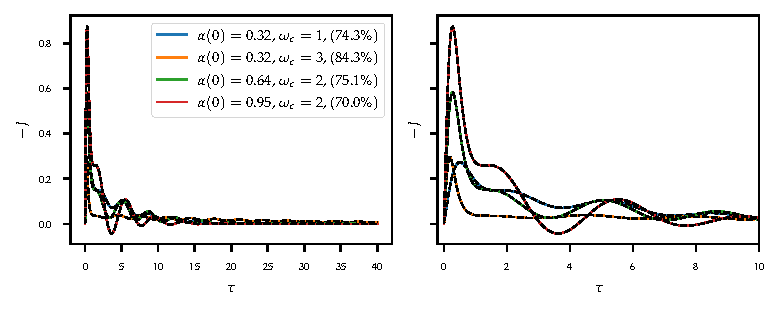
\includegraphics{figs/analytic_comp/flow_comp_zero.pdf}
  \caption{\label{fig:comp_zero_t} The bath energy flow \(-J\) for
    different parameters of the ohmic bath correlation
    function \cref{eq:ohmic_bcf}. The solid lines have been obtained
    with HOPS and the dashed lines using the analytic solution. A good
    agreement is evident visually and corroborated by the consistency
    values in the legend (see \cref{sec:meth} for an explanation).}
\end{figure}
\paragraph{Zero Temperature}
The bath energy flow \(J=∂_t\ev{H_\bath}\), from here on called simply
``the flow'' or ``bath energy flow'', for the zero temperature case
are illustrated in \cref{fig:comp_zero_t}. The results agree to a very
good accuracy, validating the findings of \cref{chap:flow}.

Although the simulations are primarily intended as a benchmark for
HOPS and a verification for the results of \cref{chap:flow} some
observations can be made in \cref{fig:comp_zero_t}. First, the flows
for different parameters all feature the characteristic spike
originating from the ``initial slip'', as explained in
\cref{sec:pure_deph} This is a quite universal feature and also shows
up on a single trajectory level suggesting that it is not strictly
related to an energy exchange with the bath but rather to the build-up
of interaction energy. This will be discussed further in
\cref{sec:prec}. \fixme{maybe a plot}The time dependence of the flow
also varies both with the shape of the BCF and the coupling
strength. For longer correlation times \(\propto 1/ω_c\) we find that
the flow initially decays much slower at the same coupling strength
(blue and orange lines) and exhibits stronger oscillations. After this
initial period the situation is reversed. For large coupling strengths
we can observe a ``backflow'' of energy out of the bath. In all cases
the flow features some oscillations and decays to zero which is
physical for the situation of a harmonic oscillator that gives all its
energy into a zero temperature bath.

The observed behaviour for longer bath memories may be qualitatively
understood by assuming that the system interacts with the same part of
the bath for a longer time and can therefore more efficiently transfer
energy. When the bath memory is short however, new interactions have
to be built up continuously which leads to a slower energy transfer.

\begin{figure}[h]
  \centering
  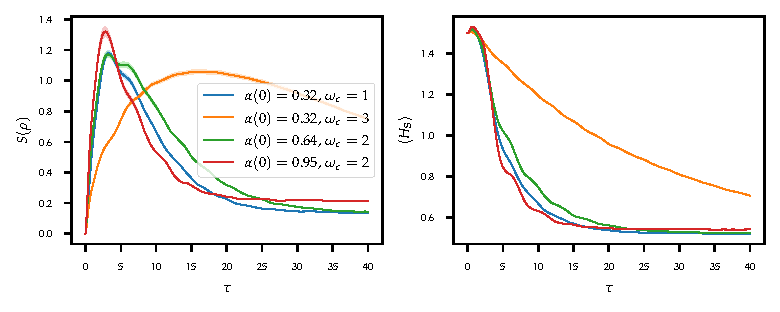
\includegraphics{figs/analytic_comp/entropy_zero.pdf}
  \caption{\label{fig:ho_zero_entropy} Left: The von Neumann entropy
    of the system state as a measure for entanglement with the
    bath. Right: The system energy as a function of time.}
\end{figure}
Note however, that the steady state is not a product state as can be
seen by the residual entropy in \cref{fig:ho_zero_entropy} in the
cases where the steady state has been approximately reached. The
stronger the coupling, the larger the entanglement. The \(α(0)=0.95\)
simulation appears to be leading to a qualitatively different steady
state than the one with the same cutoff but weaker coupling
strength. This also manifests in a higher expected system energy in
the steady state.

The time dependence of the entropy the expectation value of the system
energy is markedly different for \(ω_c=3\). Although the coupling
strength is larger than in the \(α(0)=0.32,\, ω_c=1\) case the energy
loss of the system is markedly slower and the initial energy gain is
less pronounce. This is consistent with the flow in
\cref{fig:comp_zero_t}.

The simulation was run with a hierarchy depth of \(\norm{\vb{k}} = 5\)
(simplex truncation\footnote{see \cref{sec:hops_basics}}) and a BCF
fit with \(7\) terms taken from \cite{RichardDiss} which was also used
in the analytical solution. The harmonic oscillator Hilbert space was
truncated to \(15\) dimensions. As the initial state the first excited
state of the oscillator was chosen. Some \(N=5000\) trajectories have
been computed and lead to a quite satisfactory statistical error that
is small enough to be invisible in \cref{fig:comp_zero_t}. The
normalized standard deviation of the bath energy flow follows the
usual one-over-square-root rule as is illustrated in
\cref{fig:sqrt_conv}. Even after just \(N=1000\) trajectories the
normalized statistical error is on the order of \(10^{-3}\).
\begin{figure}[h]
  \centering
  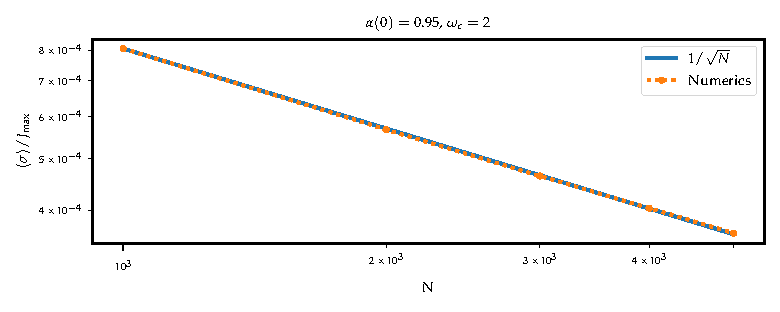
\includegraphics{figs/analytic_comp/sqrt_convergence.pdf}
  \caption{\label{fig:sqrt_conv} The (empirical) standard deviation
    (the statistical error) of the flow for the last configuration in
    \cref{fig:comp_zero_t} normalized by the maximum absolute value of
    \(J\).}
\end{figure}
\begin{figure}[h]
  \centering
  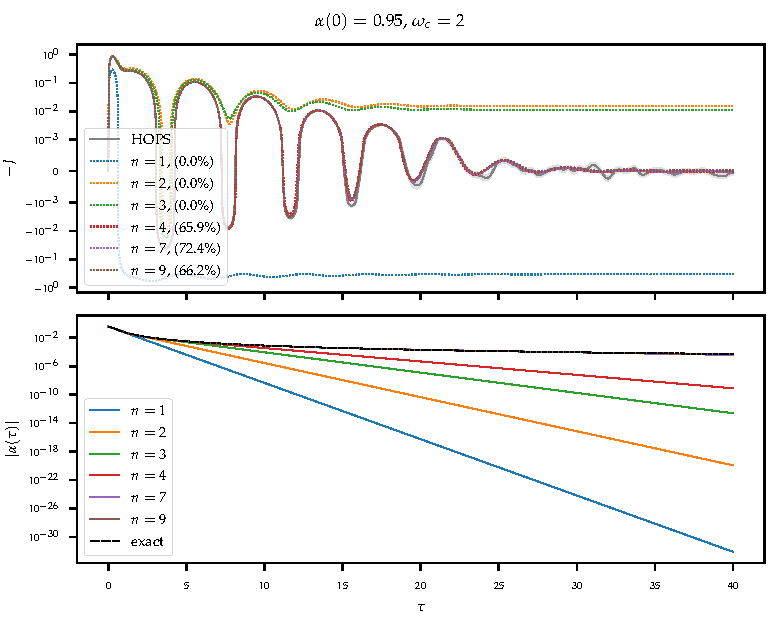
\includegraphics{figs/analytic_comp/analytical_terms_important.pdf}
  \caption{\label{fig:analytical_terms_important} Upper Panel: The analytical
    solution for the zero temperature bath energy flow using different
    numbers of terms in the BCF expansion in a symmetric logarithmic
    scale. For \(7\) terms the consistency (number in parentheses)
    with the numerical solution is best. Lower Panel: The absolute
    value of the approximated bath correlation function.}
\end{figure}
The analytical solution is quite sensitive to the quality of the BCF
expansion.  While one might expect that choosing the same number of
terms in the expansion for the analytical solution as was used for the
HOPS simulation, there still remains a systematic difference between
HOPS and the analytical solution, as the stochastic processes is
sampled using the full bath correlation function and more intricate
approximations~\cite{RichardDiss}.  Nevertheless, the best agreement
is found for using the same number expansion terms in both HOPS and
the analytical solution as is illustrated in
\cref{fig:analytical_terms_important}. Note that the consistency value
given in \cref{fig:analytical_terms_important} is different from the
one in \cref{fig:comp_zero_t}, as here a separate fit was made rather
than using the fit from \cite{RichardDiss}.

Interestingly, the solutions using a BCF expansion with three terms or
fewer lead to an unphysical non-zero steady state bath energy
flow. Considering specifically the case of one expansion this may be
related to the fact that now the BCF  term so that
\(α(τ)=G \exp(-Wτ)\) is related to a Lorentzian spectral density that
also includes unphysical negative frequencies.

\fixme{additional curve in plot, idea: start in the zero state ->
  product state is not the steady state, maybe longer times}

\paragraph{Finite Temperature}
\begin{figure}[t]
  \centering
  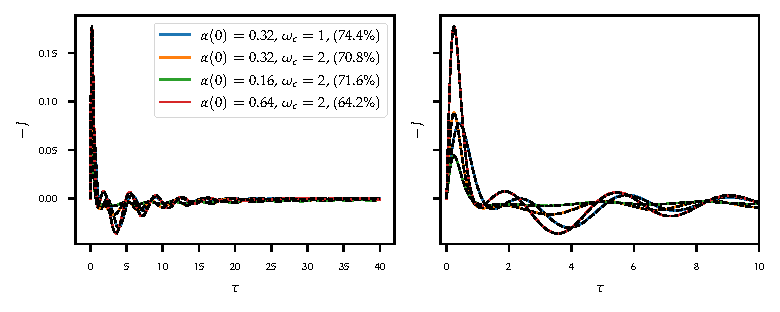
\includegraphics{figs/analytic_comp/flow_comp_nonzero.pdf}
  \caption{\label{fig:comp_finite_t} The bath energy flow \(-J\) of
    the quantum Brownian motion model for different parameters of the
    ohmic bath correlation function \cref{eq:ohmic_bcf} in the finite
    temperature \(T=1\) case. The presentation is equivalent to
    \cref{fig:comp_zero_t}.}
\end{figure}
The results for the finite temperature case are illustrated in
\cref{fig:comp_finite_t} for a temperature of \(T=1\). The setup was
otherwise equivalent to the zero temperature simulations, except for
the number of trajectories which was chosen to be \(N=10^5\).  Again
the high consistency values suggest that the findings of
\cref{chap:flow} are valid. The last case (\(α(0)=0.64,\, ω_c=2\)),
falls just short of the \(68\%\) mark, but agrees very well
visually. It is very probable, that simply more samples are required.

We find a similar behaviour as in the zero temperature case, but this
time with a more pronounced flow out of the bath. For higher coupling
strengths, the flow amplitude is higher, as is also the case for lower
cutoffs.

One potentially contestable point in \cref{chap:flow} was the
appearance of the time derivative of the thermal stochastic process in
\cref{eq:pureagain}. The numerical method which is used to sample the
stochastic processes allows for a straight forward implementation of
this derivative so that no numerical derivatives are required and
there appears to be no problem.

As the dimensionality of the Monte Carlo integral underlying the
NMQSD/HOPS formalism is increased by the ``Stochastic Hamiltonian''
method, we observe markedly slower convergence as the variance of the
individual trajectories is higher.  In \label{fig:cons_dev_finite} the
convergence behaviour, as well the consistency with increasing
trajectory count are shown and this behaviour is observed. We also
find that in the more challenging regimes of stronger coupling or
longer bath correlation times the behaviour of the convergence is more
volatile, dipping into regions of inconsistency even at high sample
counts. While the mean difference between the numerical and the
analytical flow is always below the mean statistical error, larger
fluctuations can occur at certain points in time when a new region of
the probability space is sampled.

\begin{figure}[p]
  \centering
  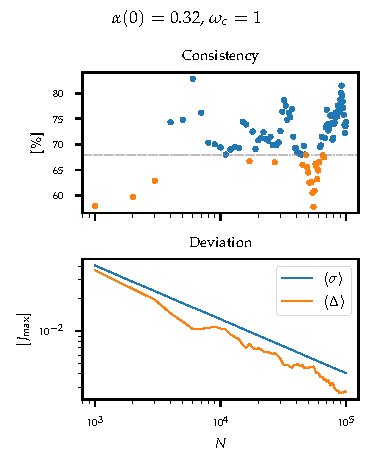
\includegraphics{figs/analytic_comp/consistency_development_0.pdf}
  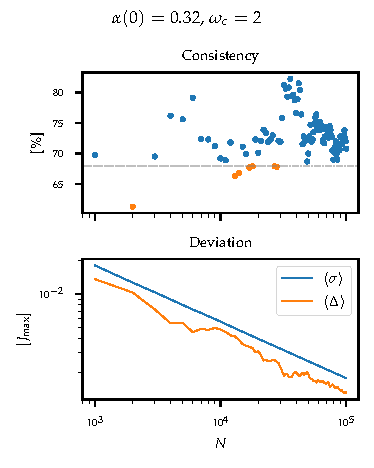
\includegraphics{figs/analytic_comp/consistency_development_1.pdf}
  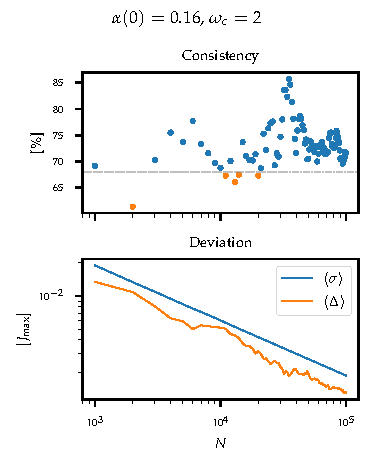
\includegraphics{figs/analytic_comp/consistency_development_2.pdf}
  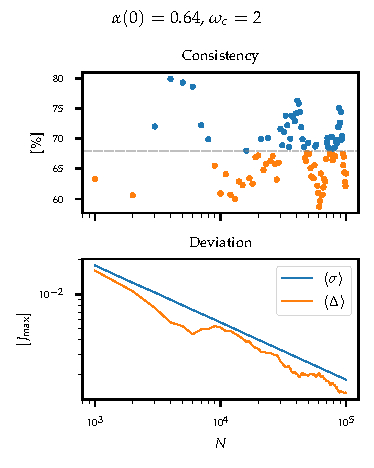
\includegraphics{figs/analytic_comp/consistency_development_3.pdf}
  \caption{\label{fig:cons_dev_finite} The convergence of the flows of
    \cref{fig:comp_finite_t} with increasing trajectory count. The upper
    panels show the consistency, where the grey marks the \(68\%\)
    threshold for consistency. The lower panel shows the time averaged
    values of the statistical error \(\ev{σ}\) and the deviation from
    the analytical result \(\ev{Δ}\) by the maximum absolute value of
    \(J\).}
\end{figure}

% The advantage of the ``Stochastic Hamiltonian'' method for finite
% temperature (see \cref{eq:thermalh}) is that one doesn't have to deal
% with the finite temperature BCF that does decay markedly slower than
% its zero temperature counterpart as is illustrated in
% \cref{fig:bcf_decay}. Generically, more terms in the BCF expansion
% would be required to capture the algebraic decay appropriately.

% \begin{figure}[t]
%   \centering
%   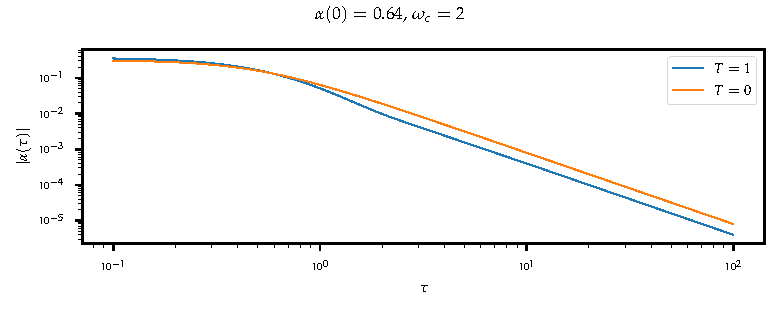
\includegraphics{figs/analytic_comp/bcf_decay.pdf}
%   \caption{\label{fig:bcf_decay} The absolute value of the Ohmic BCF
%     used in the last simulation of \cref{fig:comp_zero_t}.}
% \end{figure}

\subsection{Two Oscillators, Two Baths}
\label{sec:twoosccomp}

The model of \cref{sec:oneosc} was generalized to two oscillators
coupled to two separate baths in \cref{sec:twoosc} and
\cref{eq:hamiltonian_two_bath}. In this section we simulate this model
and compare the results with the analytical solution.

For simplicity, the parameters were chosen symmetric so that the
frequencies of both oscillators are the same \(Ω=Λ=1\). As before,
\(Ω\) defines the energy unit. The zero temperature bath correlation
functions of both baths were chosen identically with a cutoff
frequency \(ω_c=2\). The intra-oscillator coupling was chosen as
\(γ=0.5\). The hierarchy was truncated so that \(\abs{\vb{k}}\leq 3\) and a BCF
expansion with five terms was chosen to limit memory demands.
\fixme{mention number of samples}

To limit the variance the temperature of one of the baths was set to
zero, so that only one thermal stochastic process was introduced. The
other bath was chosen to have \(T=0.6\). The ground state of the
system Hamiltonian \(\ket{0}\otimes \ket{0}\) was chosen as the
initial state of the oscillators.

The main challenge of simulating the model \cref{eq:hamiltonian_two_bath} is
the dimension of the system Hilbert space which is constrained by the
available memory. In the simulation discussed here, each oscillator
was truncated at \(9\) levels leading to \(9^2 = 81\) dimensions in
total\footnote{This is a naive method of truncation, but sufficient
  for the purposes of this work.}. The effect of a too drastic
truncation of the system Hilbert space can be seen in
\cref{fig:insufficient_levels}. At the temperature chosen the mean
level occupation of a harmonic oscillator is given by the Bose distribution
\begin{equation}
  \label{eq:harm_mean_occ}
  \ev{n} = \frac{1}{\eu^{Ωβ}-1} \approx 0.23 < 1.
\end{equation}
Nevertheless, quite more than two levels are required per
oscillator. This may be due to a required minimal resolution of the
position operators that occur in the model
\cref{eq:hamiltonian_two_bath} which is formulated with position space
in mind.

The final result can be studied in \cref{fig:sufficient_levels}. We
find good, but not excellent agreement. Based on the results of
\cref{sec:oneosccomp} however, it can be argued that this result is
sufficient to corroborate the validity of the results of
\cref{sec:multibath}. With more computational effort and fine-tuning
of parameters a better agreement between the analytical and the
numerical results may be achieved.
\begin{figure}[h]
  \centering
  \begin{subfigure}[t]{.49\linewidth}
    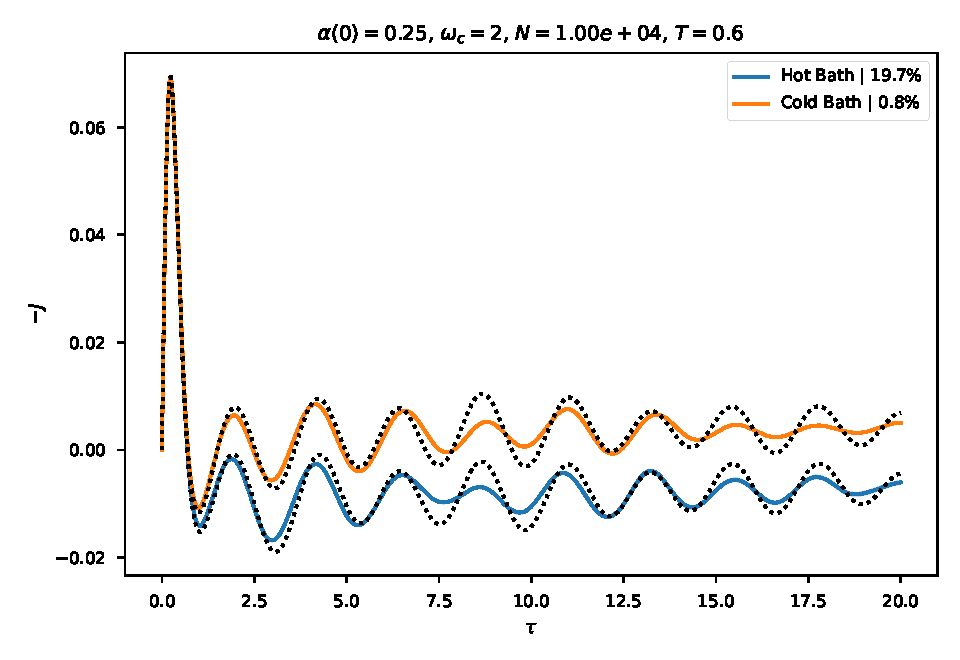
\includegraphics{figs/analytic_comp/comparison_two_5bcf_5ho.pdf}
    \caption{\label{fig:insufficient_levels}\(\dim\hilb_\sys=25\).}
  \end{subfigure}
  \begin{subfigure}[t]{.49\linewidth}
    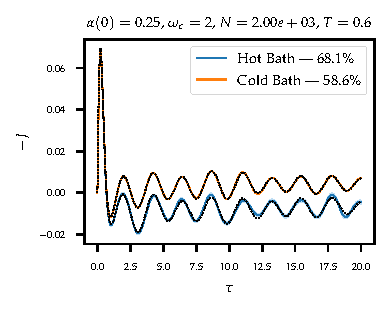
\includegraphics{figs/analytic_comp/comparison_two.pdf}
    \caption{\label{fig:sufficient_levels}\(\dim\hilb_\sys=81\).}
  \end{subfigure}
  \caption{\label{fig:comp_two_bath} The bath energy flows for
    the model \cref{eq:hamiltonian_two_bath}, where the dashed lines
    correspond to the analytical solutions.}
\end{figure}

\Cref{fig:comp_two_bath} exhibits some interesting features. The
initial slip peak in the bath energy flows is identical for both baths
and independent of temperature as suggested by the discussion in
\cref{sec:pure_deph}. As is expected, the hot bath looses energy and
the cold bath gains energy, while this process is modulated by the
intra-oscillator coupling. It follows from the analytical solution
that eventually a steady state without oscillations will be reached.

Interestingly, the zero temperature bath flow converges very much
faster than the finite temperature flow despite the whole system being
connected, at least indirectly, to the hot bath. The reason for this
is that the derivative of the thermal stochastic process \(\dot{ξ}\)
dominates the variance of the flow for each trajectory. This is also
the reason that expressions depending on the hierarchy states rather
than time derivatives of stochastic processes are preferred as
discussed in \cref{sec:general_obs}.


\fixme{show simulation with insufficient HO levels}


\section{Precision Simulations for a Single Bath}
\label{sec:prec}
\begin{itemize}
\item consistency
\item dependency upon BCF and coupling strength
\end{itemize}

\section{Modulation of System and Interaction for a Single Bath}
\label{sec:singlemod}
\begin{itemize}
\item quantum friction
\item non-markovianity in the energy shovel
\item resonance effects
\item nonuniform level spacing, three level system
\item \ldots
\end{itemize}


\section{Anti Zeno Engine}
\label{sec:antizeno}


\section{Miscellaneous Demonstrations of the Capabilities of HOPS}
\label{sec:miscdemo}
Very short mention of some results from ``side projects'' if I have
the time to include them.

\begin{itemize}
\item two qubits coupled to each other -> steady state flow
\item otto cycle
\item rotating engine
\end{itemize}
\section{Some Ideas for future Work}
\begin{itemize}
\item ... list all those nice papers ...
\item the third law
\item look more deeply into the peculiarities in \cref{sec:oneosccomp}
\end{itemize}
